\chapter{Deep Learning for Text Classification}

FFN structure has problems when dealing with text representations:
\begin{itemize}
	\item Texts are composed of discrete objects (words, characters), FFN expect
numerical inputs
	\item Texts lenghts are variable, input size of a FFN is fixed
\end{itemize}
Possible solutions:
\begin{itemize}
	\item Word embeddings to convert text sequences into numerical data
	\item Recurrent networks or other alternatives to process sequences
\end{itemize}
These problems appear in other objects: speech, handwritten text, general
temporal sequences, protein chains, video, large images,\dots

\section{Word Embeddings}

\begin{paracol}{2}
   
   Discrete symbols can be encoded by assigning them one or more numbers
   E.g., ``a'' $\rightarrow 1$, ``b'' $\rightarrow 2$, \dots
   
   To fit the natural input of neural networks, many representations are possible:
   \begin{itemize}
      \item One-hot encoding (or local) - a binary vector, size of vocabulary, 1 in the position of the symbol, 0 in the rest of positions
      \item Distributed - binary encoding of an assigned natural number
      \item Embedding - real values vector of a predefined dimension D
   \end{itemize}
      
   \switchcolumn

   \begin{figure}[htbp]
      \centering
      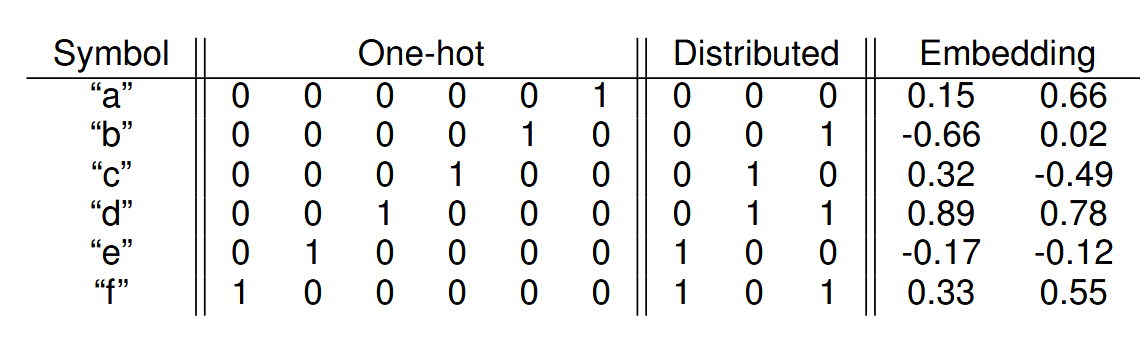
\includegraphics{images/09/embeddings.png}
      \caption{Word Embeddings}
      \label{fig:09/embeddings}
   \end{figure}

\end{paracol}

\section{Word Embeddings: Word2Vec}
Word2Vec is a method to learn word embeddings from large text corpora.
It uses a shallow neural network to predict the context of a word or the word itself given its
context. The two main architectures are:
\begin{itemize}
   \item Continuous Bag of Words (CBOW): Predicts a word given its context.
   \item Skip-Gram: Predicts the context given a word.
\end{itemize}


\section{RNN: Recurrent Neural Networks}
Recurrent Neural Networks (RNNs) are a type of neural network designed to handle sequential data, such as text or time series. They maintain a hidden state that captures information about previous inputs, allowing them to process sequences of variable length.
Simple RNN have some problems:
\begin{itemize}
   \item Output depends on past information
   \begin{itemize}
      \item It depends on more recent or older information according the moment
      \item If a balance is not kept, recent information dominates
   \end{itemize}
\item  Errors in backward propagation tend to vanish (tend to 0) or oscilate (do not allow convergence)
\end{itemize}

Solution: units with dedicated parts (gates) to different inputs and outputs
\begin{itemize}
	\item \textit{Long-Short Term Memories} (\textbf{LSTM})
	\item \textit{Gated Recurrent Units} (\textbf{GRU})
\end{itemize}

\subsection{Encoders and Decoders}
Encoders and decoders are architectures used in sequence-to-sequence tasks, such as machine translation  or text summarization. \ul{The encoder processes the input sequence and compresses it into a fixed-size context vector}, while \ul{the decoder generates the output sequence from this context vector}.

\begin{itemize}
	\item \textbf{Encoder}: from input sequence $x$ generates context representations
sequence $h^e$
	\item \textbf{Context}: $c = f(h^e_n)$, keeps input essence
	\item \textbf{Decoder}: from context $c$ generates output sequence $y$
Non-autoregressive in training, autoregressive in production
\end{itemize}

Hay el problema del \textit{bottleneck} en el contexto, que puede ser
resuelto con \textbf{attention mechanisms}.
El problema del \textit{bottleneck} es que la información de la secuencia de entrada se comprime en un vector de contexto, lo que puede llevar a una pérdida de información importante, especialmente en secuencias largas.

\textbf{Transformers} 

Transformers are a type of neural network architecture that uses self-attention mechanisms to process sequences. They are particularly effective for tasks like machine translation, text summarization, and language modeling. Transformers consist of an encoder and a decoder, both composed of multiple layers of self-attention and feed-forward networks.

\begin{itemize}
	\item Query: current input where
attention is computed
	\item Key: context compared to
current input
	\item Value: final attention value
\end{itemize}